\documentclass{article}
\usepackage{graphicx, mathtools, amsmath, amssymb, float, fancyhdr}
\usepackage[symbol]{footmisc}

\renewcommand{\thefootnote}{\fnsymbol{footnote}}

\graphicspath{{Images/}}

\setlength{\oddsidemargin}{0in}
\setlength{\textwidth}{6.5in}
\setlength{\topmargin}{-.55in}
\setlength{\textheight}{9in}
\pagestyle{fancy}

\fancyfoot{}
\fancyhead[L]{MATH 5430}
\fancyhead[R]{\thepage}


\begin{document}

\begin{center}
    {\Large Homework 2}
    \vspace{0.5 cm}

    {\large Michael Nameika}
\end{center}

\section*{Section 1.5 Problems}
\begin{itemize}
    \item[\textbf{31}.] Discuss the equation $\dot{x} = x^2 - t$.
    \newline\newline
    \textit{Discussion:} The equation $\dot{x} = x^2 - t$ is a Riccati type equation. Similar to the example in the text, we have that $f(x,t) = x^2 - t \in C^1(\mathbb{R}^2, \mathbb{R})$ and so a unique solution exists locally near $(x_0, t_0)$. Notice that the equation has nullclines whenever $x(t) = \pm \sqrt{t}$. Note that
    \begin{align*}
        f(x,t) &> 0 \:\:\:\: \text{ when  }\:\: x(t) > \sqrt{t}\\
        f(x,t) &< 0 \:\:\:\: \text{ when  }\:\: -\sqrt{t} < x(t) < \sqrt{t}\\
        f(x,t) &> 0 \:\:\:\: \text{ when  }\:\: x(t) < -\sqrt{t}
    \end{align*}
    Thus, $x(t)$ can move from region I to region II, or move from region III to region II, but once in region II, will remain in region II, as can be seen in the following figure:
    \begin{figure}[H]
        \centering
        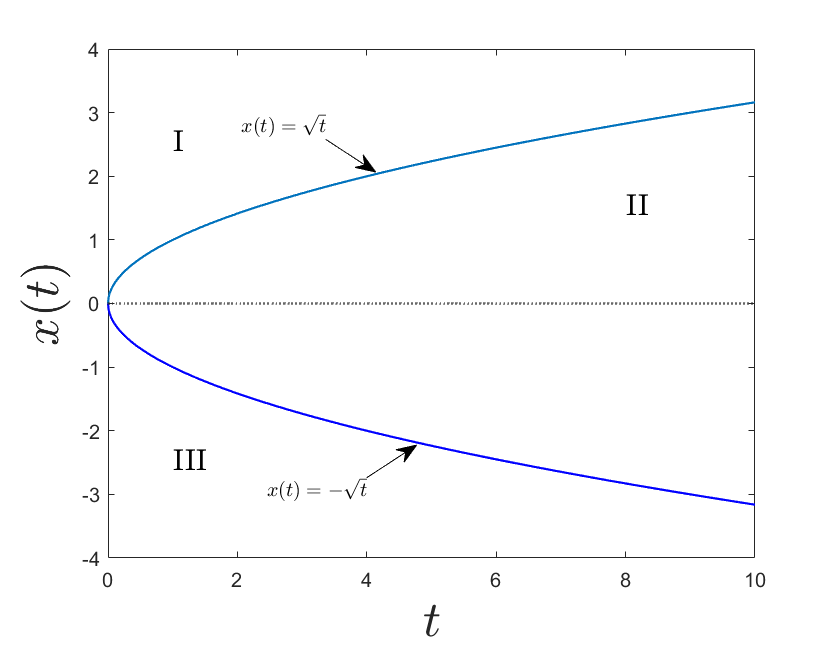
\includegraphics[scale = 0.4]{discussionPlot.png}
        \caption{Region splitting :)}
    \end{figure}
    Note that as $t \to \infty$, we have that if $x(t)$ is in region I, $x(t)$ will either diverge to $+\infty$ or enter into region II. If $X(t)$ is in region II, then $x(t)$ will diverge to $-\infty$, but cannot diverge in finite time since $x(t)$ is bounded below by $-\sqrt{t}$. Finally, if $x(t)$ is in region III, then $x(t)$ will eventually cross over into region II and diverge to $-\infty$.
    
\end{itemize}


\section*{Section 2.1 Problems}
\begin{itemize}
    \item[\textbf{2}.] Let $X$ be a Banach space. Show that the norm, vector addition, and multiplication by scalars are continuous. That is, if $f_n \to f$, $g_n \to g$, and $\alpha_n \to \alpha$, then $\|f_n\| \to \|f\|$, $f_n + g_n \to f + g$, and $\alpha_nf_n \to \alpha f$. 
    \newline\newline
    \textit{Proof:} To begin, fix $\varepsilon > 0$. We will begin by showing $\|f_n\| \to \|f\|$. By definition of convergence in a normed space, we have for some natural number $N_1$, whenever $n > N_1$,
    \[\|f_n - f\| < \varepsilon\]
    but by the reverse triangle inequality (see previous submission), we have
    \[|\|f_n\| - \|f\|| \leq \|f_n - f\|\]
    hence
    \[|\|f_n\| - \|f\|| < \varepsilon\]
    so that $\|f_n\| \to \|f\|$. Now, for some other natural number $N_2$, whenever $n > N_2$, we have
    \[\|f_n - f\| < \frac{\varepsilon}{2} \hspace{0.5cm} \|g_n - g\| < \frac{\varepsilon}{2}\]
    \begin{align*}
        \|(f_n + g_n) - (f - g)\| &= \|(f_n - f) + (g_n - g)\|\\
        &\leq \|f_n - f\| + \|g_n - g\|\\
        &< \frac{\varepsilon}{2} + \frac{\varepsilon}{2}\\
        &= \varepsilon.
    \end{align*}
    Hence, $f_n + g_n \to f + g$. Now consider
    \begin{align*}
        \|\alpha_n f_n - \alpha f\| &= \|\alpha_n f_n - \alpha_n f + \alpha_n f - \alpha f\|\\
        &\leq \|\alpha_nf_n - \alpha_n f\| + \|\alpha_n f - \alpha f\|\\
        &= |\alpha_n|\|f_n - f\| + |\alpha_n - \alpha|\|f\| \tag*{(Homogeneity of the norm)}
    \end{align*}
    and since $\alpha_n \to \alpha$, $\{\alpha_n\}$ is a bounded sequence. That is, there exists some $M > 0$ such that 
    \[|\alpha_n| \leq M\]
    for all $n$. Now, for some $N_3 \in \mathbb{N}$, we have that, whenever $n > N_3$\footnote[2]{If $\|f\| = 0$, we simply use $\|f_n - f\| < \frac{\varepsilon}{2M}$ since $\|f\||\alpha_n - \alpha| = 0$.},
    \[\|f_n - f\| < \frac{\varepsilon}{2M} \hspace{0.5cm} |\alpha_n - \alpha| < \frac{\varepsilon}{2\|f\|}\]
    so that, from our work above, we have
    \begin{align*}
        |\alpha_n|\|f_n - f\| + |\alpha_n - \alpha|\|f\| &< M\frac{\varepsilon}{2M} + \|f\|\frac{\varepsilon}{2\|f\|}\\
        &= \frac{\varepsilon}{2} + \frac{\varepsilon}{2}\\
        &= \varepsilon.
    \end{align*}
    Hence, $\alpha_nf \to \alpha f$.
\end{itemize}

\section*{Section 2.2 Problems}
\begin{itemize}
    \item[\textbf{6}.] Are the following functions Lipschitz continuous near 0? If yes, find a Lipschitz constant for some interval containing 0.
    \begin{itemize}
        \item[(i)] $f(x) = \frac{1}{1 - x^2}$.
        \newline\newline
        For any closed interval $[a,b]$ ($a > -1, b < 1$) containing 0, since $f(x) \in C^1[a,b]$, using Taylor's theorem, we have
        \[|f(x) - f(x_0)| = |f'(\xi)||x - x_0|\]
        for $x,x_0 \in [a,b]$ and $\xi \in [x,x_0]$. Then since 
        \[f'(\xi) = \frac{2\xi}{(1 - \xi^2)^2}\]
        and since $f'$ is monotonically increasing on, we have
        \[|f'(\xi)| \leq \frac{2b}{(1 - b^2)^2}\]
        so that
        \begin{align*}
            |f(x) - f(x_0)| &\leq \frac{2b}{(1 - b^2)^2} (b - a).
        \end{align*}
        Alternatively, on any compact interval $[a,b] \subset (-1,1)$, since $f \in C^1[a,b]$, $f$ is Lipschitz over $[a,b]$.
        
        
        \item[(ii)] $f(x) = |x|^{1/2}$.
        \newline\newline
        I claim $f$ is not Lipschitz near zero. To see this, take $[a,b]$ an interval that contains zero. If $f$ is Lipschitz, then there exists some constant $K > 0$ such that
        \[|f(x) - f(y)| \leq K|x - y|\]
        In particular, take $y = 0$. Then we have
        \begin{align*}
            \sqrt{|x|} &\leq K|x|\\
            \frac{1}{\sqrt{|x|}} &\leq K
        \end{align*}
        but as $x \to 0$, $\frac{1}{\sqrt{|x|}} \to \infty$, so $K$ is unbounded. Hence $f$ is not Lipschitz near zero.
        

        \item[(iii)] $f(x) = x^2 \sin(\frac{1}{x})$.
        \newline\newline
        (Can we assume that $f(0) = 0$ so the discontinuity is removed?) I claim $f(x)$ is globally Lipschitz. By the mean value theorem, for $x,x_0 \in \mathbb{R}$, we have that there exists some $\xi \in (x,x_0)$ such that
        \[|f(x) - f(x_0)| = |f'(\xi)||x - x_0|\]
        and 
        \[f'(x) = 2x\sin\left(\frac{1}{x}\right) - \cos\left(\frac{1}{x}\right)\]
        and so
        \begin{align*}
            |f'(x)| &= \left|2x\sin\left(\frac{1}{x}\right) - \cos\left(\frac{1}{x}\right)\right|\\
            &\leq 2\left|x\sin\left(\frac{1}{x}\right)\right| + \left|\cos\left(\frac{1}{x}\right)\right|\\
            &\leq 2\left|x\sin\left(\frac{1}{x}\right)\right| + 1\\
            &\leq 2 + 1\\
            &= 3
        \end{align*}
        Hence, $|f'(x)| \leq 3$ for all $x \in \mathbb{R}$. Then 
        \[|f(x) - f(x_0)| \leq 3|x - x_0|\]
        so that $f$ is globally Lipschitz with Lipschitz constant 3.
        \newline

        Note: Since $\lim_{x \to 0} x\sin\left(\frac{1}{x}\right) = 0$ by the squeeze theorem, and 
        \begin{align*}
            \lim_{x \to \pm \infty}x\sin\left(\frac{1}{x}\right) &= \lim_{x \to \pm \infty} \frac{\sin\left(\frac{1}{x}\right)}{\frac{1}{x}}\\
            &= 1.
        \end{align*}
        

        
    \end{itemize}


    \item[\textbf{8}.] Apply the Picard iteration to the first-order equation
    \[\dot{x} = 2t - 2\sqrt{\max(0,x)}, \:\: x(0) = 0.\]
    Does it converge?
    \newline\newline
    \textit{Soln.} Applying the Picard iteration to the above equation, we have $x_0(t) = 0$ and 
    \begin{align*}
        x_1(t) &= 0 + \int_0^t (2s - 2\sqrt{\max(0, 0)})ds\\
        &= \int_0^t 2s ds\\
        &= t^2
    \end{align*}
    and
    \begin{align*}
        x_2(t) &= \int_0^t (2s - 2\sqrt{\max(0, s^2})ds\\
        &= \int_0^t (2s - 2s)ds\\
        &= \int_0^t 0 ds\\
        &= 0.
    \end{align*}
    We now fall into a cycle. It is clear from here that our $n^{\text{th}}$ Picard iteration will have the following form:
    \[x_n(t) = \begin{cases}
        0 & n \equiv 0 \mod 2\\
        t^2 & n \equiv 1 \mod 2
    \end{cases}\]
    So that it does not converge.
    
    
\end{itemize}

\section*{Section 2.4 Problems}
\begin{itemize}
    \item[\textbf{12}.]  Show (2.38). (Hint: Introduce $\tilde{\psi}(t) = \psi(t) + \frac{\gamma}{\beta}$.)
    \newline\newline
    \textit{Proof:} Suppose 
    \[\psi(t) \leq \alpha + \int_0^t (\beta \psi + \gamma) ds.\] 
    Let $\tilde{\psi}(t) = \psi(t) + \frac{\gamma}{\beta}$. Then the above inequality becomes
    \begin{align*}
        \tilde{\psi}(t) - \frac{\gamma}{\beta} &\leq \alpha + \int_0^t \beta \tilde{\psi}(s)ds\\
        \tilde{\psi}(t) &\leq \alpha + \frac{\gamma}{\beta} + \int_0^t \beta \tilde{\psi}(s)ds
    \end{align*}
    Since $\alpha + \tfrac{\gamma}{\beta}$ is just a constant, call it $\tilde{\alpha}$. Then the above inequality becomes
    \[\tilde{\psi}(t) \leq \tilde{\alpha} + \int_0^t \beta \tilde{\psi}(s)ds.\]
    Then by (2.36), we have
    \[\tilde{\psi}(t) \leq \tilde{\alpha}e^{\beta t}\]
    which, using $\tilde{\alpha} = \alpha + \tfrac{\gamma}{\beta}$ and $\tilde{\psi} = \psi + \tfrac{\gamma}{\beta}$, we have
    \begin{align*}
        \psi(t) &\leq \left(\alpha + \frac{\gamma}{\beta}\right)e^{\beta t} - \frac{\gamma}{\beta}\\
        &= \alpha e^{\beta t} + \frac{\gamma}{\beta}(e^{\beta t} - 1)
    \end{align*}
    so that
    \[\psi(t) \leq \alpha e^{\beta t} + \frac{\gamma}{\beta}(e^{\beta t} - 1)\]
    which is what we wanted to show.
\end{itemize}

\section*{Section 2.6 Problems}
\begin{itemize}
    \item[\textbf{18}.] Show that Theorem 2.17 is false (in general) if the estimate is replaced by
    \[|f(t,x)| \leq M(T) + L(T)|x|^{\alpha}\]
    with $\alpha > 1$.
    \newline\newline
    \textit{Proof:} Consider the IVP 
    \[\dot{x} = 1 + x^2, \:\:\:\:\: x(0) = 0\]
    Clearly, the solution to this equation is $x(t) = \tan(t)$, and since $t_0 = 0$, we have that the maximum interval where the IVP is satisfied is $t \in \left(-\tfrac{\pi}{2}, \tfrac{\pi}{2}\right)$ since $\tan(t)$ cannot be continuously extended beyond this interval. But notice
    \[|f(t,x)| \leq 2 + |x|^2\]
    so that theorem 2.17 is false in general if $\alpha > 1$.
\end{itemize}

\section*{Extra}
Show that the supremum norm in Eq. (2.3) is indeed a norm.
\newline\newline
\textit{Proof:} Let $x(t) \in C(I)$. Then for a fixed $t \in I$, we have
\[0 \leq |x(t)|\]
hence,
\[0 \leq \sup_{t \in I} |x(t)|\]
and notice that $\sup_{t \in I} |x(t)| = 0$ only if $x(t) \equiv 0$, for if there exists some value of $s \in I$ where $x(s) \neq 0$, then $|x(s)| > 0$, so that $\sup_{t \in I} |x(t)| > 0$. Thus, nonnegativity holds. Let $\alpha$ be an arbitrary scalar. Then
\begin{align*}
    \|x\| &= \sup_{t \in I} |\alpha x(t)|\\
    &= \sup_{t \in I} |\alpha| |x(t)|
\end{align*}
and since $\sup(a X) = a\sup(X)$ for $a > 0$, we have
\begin{align*}
    \sup_{t \in I} |\alpha| |x(t)| &= |\alpha| \sup_{t \in I} |x(t)|\\
    &= |\alpha| \|x\|\\
    \implies \|\alpha x\| &= |\alpha| \|x\|
\end{align*}
so homogeneity holds. To show the triangle inequality holds, let $x, y \in C(I)$ and notice, for a fixed $t \in I$,
\begin{align*}
    |x(t) + y(t)| &\leq |x(t)| + |y(t)|\\
    &\leq \sup_{t \in I} |x(t)| + \sup_{t \in I} |y(t)|.
\end{align*}
Then $\sup_{t \in I} |x(t)| + \sup_{t \in I} |y(t)| = \|x\| + \|y\|$ is an upper bound for $|x(t) + y(t)|$ for all $t$, hence
\begin{align*}
    \sup_{t\in I}|x(t) + y(t)| &\leq \sup_{t \in I} |x(t)| + \sup_{t \in I} |y(t)|\\
    \implies \|x + y\| &\leq \|x\| + \|y\|
\end{align*}
so the triangle inequality holds. Thus, the supremum norm is indeed a norm.

\end{document}
